\section{Linear algebra}

Linear Algebra problems can be classified into two types.
On one side we have dense problems.
These problems are numerically stable but need to be small,
around ten hundred unknowns because of memory and computation limitations.
On the other side we have sparse problems which can handle billions of unknowns
but they have numerical problems.


\subsection{Dense linear algebra}
Dense Linear Algebra optimization has been studied for a long time\ref{42}.
Most common techniques are cache blocking, SIMD vectorization ans prefetch.
These three techniques are possible because computations of Dense problems
are regular.

\subsection{Sparse linear algebra}
Unlike Dense Linear Algebra, computations of Sparse problems are irregular.
This is mainly due to the matrix storage format.
Indeed, to efficiently store non-zero values of the matrices we need to define
a storage format for the matrices that ignore zero values.
For example, one can store all non-zero values with their 2D coordinates, this
is the COO format.


\begin{figure}[!ht]
     \begin{center}
        \subfigure[Sparse matrix example]{%
            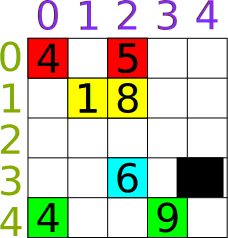
\includegraphics[width=0.25\textwidth]{matrix_format}
        }%
        \subfigure[COO storage]{%
           \label{fig:COO}
           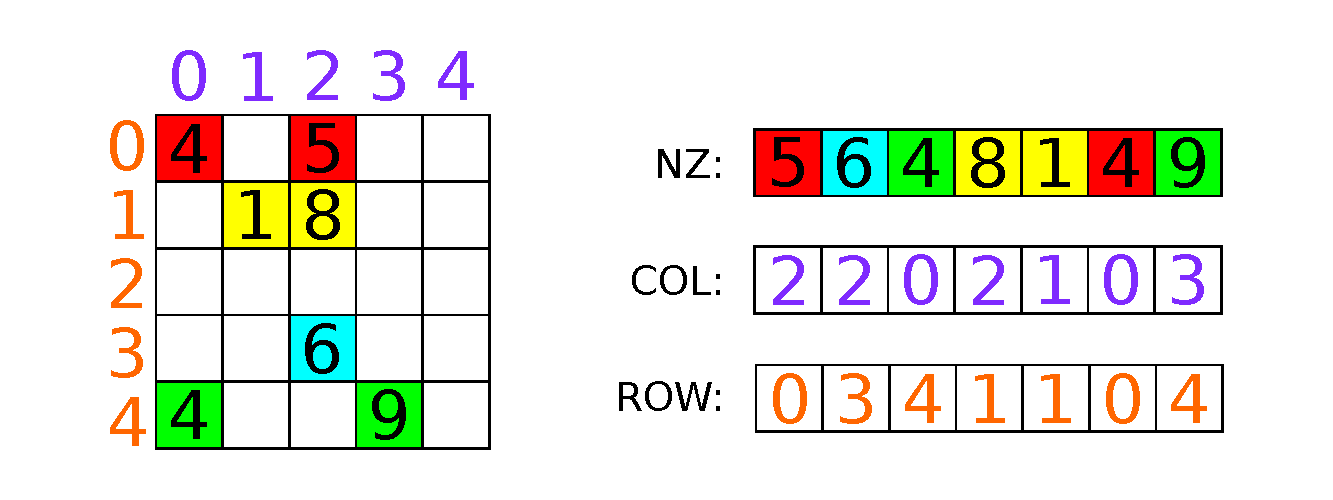
\includegraphics[width=0.35\textwidth]{COO}
        }%
        \subfigure[CSR storage]{%
            \label{fig:CSR}
            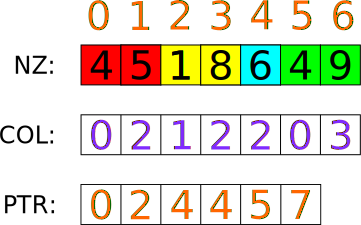
\includegraphics[width=0.35\textwidth]{CSR}
        }%
    \end{center}
    \caption{Comparison between COO and CSR matrix format storage.}
    \label{fig:matrix_storage}
\end{figure}
